\documentclass[tikz,border=2pt]{standalone}
\usepackage{pgfplots}
\pgfplotsset{compat=1.18}
\definecolor{raisedgreen}{HTML}{1A7F37}
\definecolor{regressionred}{HTML}{CF222E}
\begin{document}
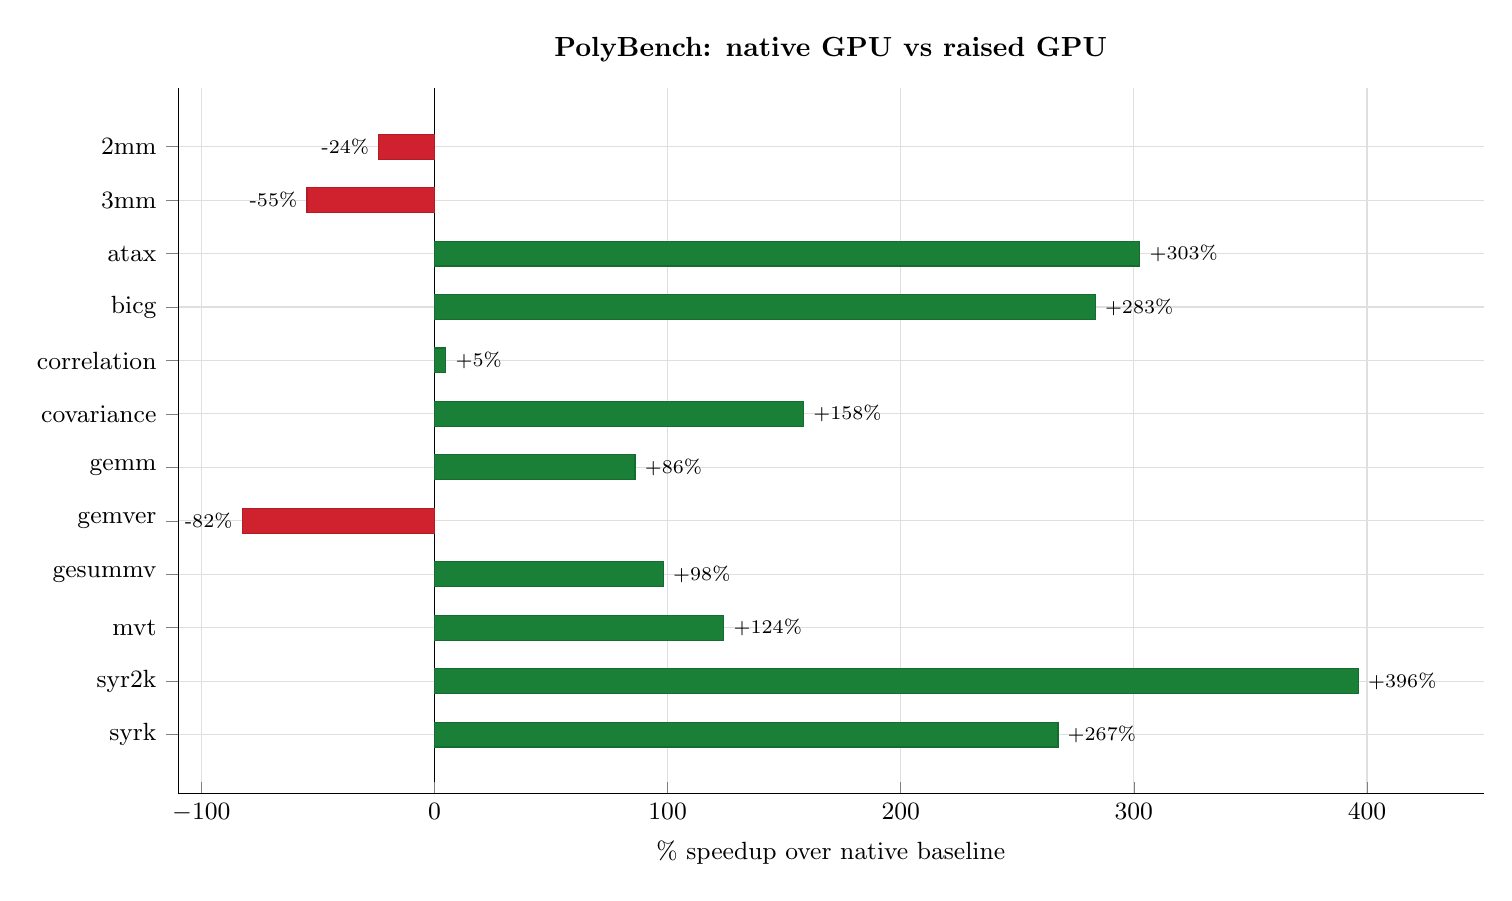
\begin{tikzpicture}
\begin{axis}[
  width=7.15in, height=4.15in,
  title={PolyBench: native GPU vs raised GPU},
  title style={font=\bfseries\normalsize},
  xbar, bar width=9pt, xmin=-110, xmax=450, xtick distance=100,
  xlabel={\% speedup over native baseline},
  ytick={0,1,2,3,4,5,6,7,8,9,10,11},
  yticklabels={{2mm},{3mm},{atax},{bicg},{correlation},{covariance},{gemm},{gemver},{gesummv},{mvt},{syr2k},{syrk}}, y dir=reverse,
  yticklabel style={font=\small}, xticklabel style={font=\small},
  label style={font=\small}, grid=major,
  major grid style={draw=gray!25}, axis lines*=left,
  extra x ticks={0}, extra x tick labels={},
  extra x tick style={grid=major,major grid style={draw=black,line width=0.7pt}},
  clip=false,
]
\addplot+[draw=raisedgreen!85!black,fill=raisedgreen,bar shift=0pt] coordinates {(302.548461375,2) (283.437848860,3) (4.839894949,4) (158.317986521,5) (86.020904524,6) (98.211818983,8) (124.152549378,9) (396.332605979,10) (267.441169584,11)};
\addplot+[draw=regressionred!85!black,fill=regressionred,bar shift=0pt] coordinates {(-23.863560445,0) (-54.690157135,1) (-82.468230666,7)};
\node[anchor=east,font=\scriptsize] at (axis cs:-23.863560445,0) {-24\%};
\node[anchor=east,font=\scriptsize] at (axis cs:-54.690157135,1) {-55\%};
\node[anchor=west,font=\scriptsize] at (axis cs:302.548461375,2) {+303\%};
\node[anchor=west,font=\scriptsize] at (axis cs:283.437848860,3) {+283\%};
\node[anchor=west,font=\scriptsize] at (axis cs:4.839894949,4) {+5\%};
\node[anchor=west,font=\scriptsize] at (axis cs:158.317986521,5) {+158\%};
\node[anchor=west,font=\scriptsize] at (axis cs:86.020904524,6) {+86\%};
\node[anchor=east,font=\scriptsize] at (axis cs:-82.468230666,7) {-82\%};
\node[anchor=west,font=\scriptsize] at (axis cs:98.211818983,8) {+98\%};
\node[anchor=west,font=\scriptsize] at (axis cs:124.152549378,9) {+124\%};
\node[anchor=west,font=\scriptsize] at (axis cs:396.332605979,10) {+396\%};
\node[anchor=west,font=\scriptsize] at (axis cs:267.441169584,11) {+267\%};
\end{axis}
\end{tikzpicture}
\end{document}
